\section{Power Series} \label{S:8.6.PowerSeries}

\vspace*{-14 pt}
\framebox{\hspace*{3 pt}
\parbox{\boxwidth}{\begin{goals}
\item What is a power series?
\item What are some important uses of power series?
\item What is the connection between power series and Taylor series?
\end{goals}} \hspace*{3 pt}}



\subsection*{Introduction}

We have noted at several points in our work with Taylor polynomials and Taylor series that polynomial functions are the simplest possible functions in mathematics, in part because  they essentially only require addition and multiplication to evaluate.  Moreover, from the point of view of calculus, polynomials are especially nice:  we can easily differentiate or integrate any polynomial.  In light of our work in Section~\ref{S:8.5.Taylor}, we now know that several important non-polynomials have polynomial-like expansions.  For example, for any real number $x$, 
$$e^x = 1 + x + \frac{x^2}{2!} + \frac{x^3}{3!} + \cdots + \frac{x^n}{n!} + \cdots.$$
As we continue our study of infinite series, there are two settings where other series like the one for $e^x$ arise:  one is where we are simply given an expression like $$1 + 2x + 3x^2 + 4x^3 + \cdots$$
and we seek the values of $x$ for which the expression makes sense, while another is where we are trying to find an unknown function $f$, and we think about the possibility that the function has expression
$$f(x) = a_0 + a_1 x + a_2 x^2 + \cdots + a_k x^k + \cdots,$$
and we try to determine the values of the constants $a_0$, $a_1$, $\ldots$.  The latter situation is explored in Preview Activity~\ref{PA:8.6}.

\begin{pa} \label{PA:8.6}
In Chapter~\ref{C:7}, we learned some of the many important applications of differential equations, and learned some approaches to solve or analyze them.  Here, we consider an important approach that will allow us to solve a wider variety of differential equations.

Let's consider the familiar differential equation from exponential population growth given by
\begin{equation} \label{eq:PA8.6_Resistance_ode}
y' = ky,
\end{equation}
where $k$ is the constant of proportionality. While we can solve this differential equation using methods we have already learned, we take a different approach now that can be applied to a much larger set of differential equations. For the rest of this activity, let's assume that $k=1$. We will use our knowledge of Taylor series to find a solution to the differential equation (\ref{eq:PA8.6_Resistance_ode}). 

To do so, we assume that we have a solution $y=f(x)$ and that $f(x)$ has a Taylor series that can be written in the form
\[y = f(x) = \sum_{k=0}^{\infty} a_kx^k,\]
where the coefficients $a_k$ are undetermined. Our task is to find the coefficients.
\ba
    \item Assume that we can differentiate a power series term by term.  By taking the derivative of $f(x)$ with respect to $x$ and substituting the result into the differential equation (\ref{eq:PA8.6_Resistance_ode}), show that the equation
\[\sum_{k=1}^{\infty} ka_kx^{k-1} = \sum_{k=0}^{\infty} a_kx^{k}\]
must be satisfied in order for $f(x) = \sum_{k=0}^{\infty} a_kx^k$ to be a solution of the DE.
\begin{activitySolution}

Differentiation term by term gives
\[y' = \sum_{k=1}^{\infty} ka_kx_{k-1}.\]
We then substitute this series into the differential equation (\ref{eq:PA8.6_Resistance_ode}) to obtain the equation

\end{activitySolution}

\item Two series are equal if and only if they have the same coefficients on like power terms. Use this fact to find a relationship between $a_1$ and $a_0$.

\begin{activitySolution}

When we write the first few terms of the series on either side of our differential equation we obtain
\[a_1 + (2)a_2x + (3)a_3x^2 + (4)a_4x^3 + \cdots + (k+1)a_{k+1}x^{k} + \cdots = a_0 + a_1x + a_2x^2 + \cdots + a_kx^k + \cdots.\]
Equating the constant terms gives us $a_1 = a_0$.

\end{activitySolution}

    \item Now write $a_2$ in terms of $a_1$. Then write $a_2$ in terms of $a_0$.

\begin{activitySolution}

Equating the degree 1 terms gives us $2a_2 = a_1$ or $a_2 = \frac{a_1}{2}$. Since $a_1 = a_0$, we have $a_2 = \frac{a_0}{2}$.

\end{activitySolution}

   \item Write $a_3$ in terms of $a_2$. Then write $a_3$ in terms of $a_0$.

\begin{activitySolution}

Equating the degree 2 terms gives us $3a_3 = a_2$ or $a_3 = \frac{a_2}{3}$. Since $a_2 = \frac{a_0}{2}$, we have $a_3 = \frac{a_0}{3!}$.

\end{activitySolution}

   \item Write $a_4$ in terms of $a_3$. Then write $a_4$ in terms of $a_0$.

\begin{activitySolution}

Equating the degree 3 terms gives us $4a_4 = a_3$ or $a_4 = \frac{a_3}{4}$. Since $a_3 = \frac{a_0}{3!}$, we have $a_4 = \frac{a_0}{4!}$.

\end{activitySolution}

    \item Observe that there is a pattern in (b)-(e). Find a general formula for $a_k$ in terms of $a_0$.

\begin{activitySolution}

Equating the degree $k-1$ terms gives us $ka_k = a_{k-1}$ or $a_k = \frac{a_{k-1}}{k}$. It appears that $a_{k-1} = \frac{a_0}{(k-1)!}$, so we have
\[a_k = \frac{a_0}{k!}.\]

\end{activitySolution}

\item Write the series expansion for $y$ using only the unknown coefficient $a_0$. From this, determine what familiar functions satisfy the differential equation (\ref{eq:PA8.6_Resistance_ode}). ({\bf Hint}: Compare to a familiar Taylor series.)

\begin{activitySolution}

Since $a_k = \frac{a_0}{k!}$ we have
\[y = a_0 \sum_{k=0}^{\infty} \frac{x^k}{k!}.\]
So the functions that satisfy the differential equation (\ref{eq:PA8.6_Resistance_ode}) are the exponential functions of the form $y = a_0e^x$.

\end{activitySolution}

\ea


\end{pa}
\afterpa 

\subsection*{Power Series} \index{power series}

As Preview Activity \ref{PA:8.6} shows, it can be useful to treat an unknown function as if it has a Taylor series, and then determine the coefficients from other information. In other words, we define a function as an infinite series of powers of $x$ and then determine the coefficients based on something besides a formula for the function. This method of using series illustrated in Preview Activity \ref{PA:8.6} to solve differential equations is a powerful and important one that allows us to  approximate solutions to many different types of differential equations even if we cannot explicitly solve them.  This approach is different from defining a Taylor series based on a given function, and these functions we define with arbitrary coefficients are given a special name.

\begin{definition} A \emph{power series} centered at $x = a$ is a function of the form
\begin{equation} \label{eq:8.6_power_series}
\sum_{k=0}^{\infty} c_k(x-a)^k
\end{equation}
where $\{c_k\}$ is a sequence of real numbers and $x$ is an independent variable.
\end{definition}
We can substitute different values for $x$ and test whether the resulting series converges or diverges. Thus, a power series defines a function $f$ whose domain is the set of $x$ values for which the power series converges.  We therefore write
\[f(x) = \sum_{k=0}^{\infty} c_k(x-a)^k.\]

It turns out that\footnote{See Exercise \ref{ex:8.5.2} in this section.}, on its interval of convergence, a power series is the Taylor series of the function that is the sum of the power series, so all of the techniques we developed in the previous section can be applied to power series as well.

\bex \label{Ex:8.6.1}
Consider the power series defined by
\[f(x) = \sum_{k=0}^{\infty} \frac{x^k}{2^k}.\]
What are $f(1)$ and $f\left(\frac{3}{2}\right)$? Find a general formula for $f(x)$ and determine the values for which this power series converges.
\eex
If we evaluate $f$ at $x=1$ we obtain the series
\[\sum_{k=0}^{\infty} \frac{1}{2^k}\]
which is a geometric series with ratio $\frac{1}{2}$. So we can sum this series and find that
\[f(1) = \frac{1}{1-\frac{1}{2}} = 2.\]
 Similarly,
\[f(3/2) = \sum_{k=0}^{\infty} \left(\frac{3}{4}\right)^k = \frac{1}{1-\frac{3}{4}} = 4.\]
In general, $f(x)$ is a geometric series with ratio $\frac{x}{2}$ and
\[f(x) = \sum_{k=0}^{\infty} \left(\frac{x}{2}\right)^k = \frac{1}{1-\frac{x}{2}} = \frac{2}{2-x}\]
provided that $-1 < \frac{x}{2} < 1$ (so that the ratio is less than 1 in absolute value). Thus, the power series that defines $f$ converges for $-2 < x < 2$.
\afterex

As with Taylor series, we define the interval of convergence of a power series (\ref{eq:8.6_power_series}) to be the set of values of $x$ for which the series converges. In the same way as we did with Taylor series, we typically use the Ratio Test to find the values of $x$ for which the power series converges absolutely, and then check the endpoints separately if the radius of convergence is finite.

\bex \label{Ex:8.6.2} Let $f(x) = \ds \sum_{k=1}^{\infty} \frac{x^k}{k^2}$. Determine the interval of convergence of this power series.
\eex
First we will draw graphs of some of the partial sums of this power series to get an idea of the interval of convergence. Let
\[S_n(x) = \sum_{k=1}^{n} \frac{x^k}{k^2}\]
for each $n \geq 1$. Figure \ref{F:8.6.Power_Series} shows plots of $S_{10}(x)$ (in red), $S_{25}(x)$ (in blue), and $S_{50}(x)$ (in green).
\begin{figure}[h]
\begin{center} \resizebox{!}{2.25in}{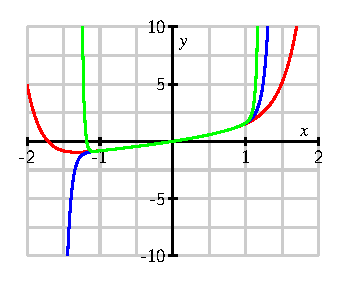
\includegraphics{figures/8_6_Power_Series.eps}}
\caption{Graphs of partial sums of the power series $\sum_{k=1}^{\infty} \frac{x^k}{k^2}$}
\label{F:8.6.Power_Series}
\end{center}
\end{figure}
The behavior of $S_{50}$ particularly highlights that it appears to be converging to a particular curve on the interval $(-1,1)$, while growing without bound outside of that interval. This suggests that the interval of convergence might be $-1 < x < 1$. To more fully understand this power series, we apply the Ratio Test to determine the values of $x$ for which the power series converges absolutely. For the given series, we have
\[a_k = \frac{x^k}{k^2},\]
so
\begin{align*}
\lim_{k \to \infty} \frac{\left| a_{k+1} \right|}{ \left| a_k \right|} &= \lim_{k \to \infty} \frac{ \frac{|x|^{k+1}}{(k+1)^2} }{ \frac{| x|^{k}}{k^2} } \\
    &= \lim_{k \to \infty} |x| \left(\frac{k}{k+1}\right)^2 \\
    &= |x| \lim_{k \to \infty}  \left(\frac{k}{k+1}\right)^2 \\
    &= |x|.
\end{align*}
Therefore, the Ratio Test tells us that the given power series $f(x)$ converges absolutely when $| x | < 1$ and diverges when $| x | > 1$.  Since the Ratio Test is inconclusive when $|x| = 1$, we need to check $x = 1$ and $x = -1$ individually.

When $x = 1$, observe that
\[f(1) = \sum_{k=1}^{\infty} \frac{1}{k^2}.\]
This is a $p$-series with $p > 1$, which we know converges.  When $x = -1$, we have
\[f(-1) = \sum_{k=1}^{\infty} \frac{(-1)^k}{k^2}.\]
This is an alternating series, and since the sequence $\left\{ \frac{1}{n^2} \right\}$ decreases to 0, the power series converges when $x=-1$ by the Alternating Series Test.  Thus, the interval of convergence of this power series is $-1 \le x \le 1$.

\afterex

\begin{activity} \label{8.6.Act1} Determine the interval of convergence of each power series.
\ba
\item $\ds \sum_{k=1}^{\infty} \frac{(x-1)^k}{3k}$
\item $\ds \sum_{k=1}^{\infty} kx^k$
\item $\ds \sum_{k=1}^{\infty} \frac{k^2(x+1)^k}{4^k}$
\item $\ds \sum_{k=1}^{\infty} \frac{x^k}{(2k)!}$
\item $\ds \sum_{k=1}^{\infty} k!x^k$
\ea

\end{activity}

\begin{smallhint}
\ba
	\item Small hints for each of the prompts above.
\ea
\end{smallhint}
\begin{bighint}
\ba
	\item Big hints for each of the prompts above.
\ea
\end{bighint}
\begin{activitySolution}
\ba
    \item We use the Ratio Test with $a_k = \frac{|x-1|^k}{3k}$:
    \begin{align*}
    \lim_{k \to \infty} \frac{ \frac{|x-1|^{k+1}}{3(k+1)} }{ \frac{|x-1|^k}{3k} } &= \lim_{k \to \infty} \frac{3k|x-1|^{k+1}}{3(k+1)|x-1|^{k}} \\
        &= |x-1| \lim_{k \to \infty} \frac{k}{k+1} \\
        &= |x-1|.
    \end{align*}
    So the power series $\ds \sum_{k=1}^{\infty} \frac{(x-1)^k}{3k}$ converges absolutely when $|x-1| < 1$ or when $0 < x < 2$ and diverges outside this interval. To completely determine the interval of convergence, we need to check what happens at the endpoints of this interval.
    \begin{itemize}
    \item When $x=0$ our power series is $\ds \sum_{k=1}^{\infty} \frac{(-1)^k}{3k}$ which is just a scalar multiple of the alternating harmonic series and so converges.
    \item When $x=2$ our power series is $\ds \sum_{k=1}^{\infty} \frac{1}{3k}$ which is just a scalar multiple of the harmonic series and so diverges.
    \end{itemize}
    Therefore, the interval of convergence of the power series $\ds \sum_{k=1}^{\infty} \frac{(x-1)^k}{3k}$ is $[0,2)$.

    \item We use the Ratio Test with $a_k = k|x|^k$:
    \begin{align*}
    \lim_{k \to \infty} \frac{ (k+1)|x|^{k+1} }{ k|x|^k } &= |x|\lim_{k \to \infty} \frac{k+1}{k} \\
        &= |x|.
    \end{align*}
    So the power series $\ds \sum_{k=1}^{\infty} kx^k$ converges absolutely when $|x| < 1$ or when $-1 < x < 1$ and diverges outside this interval. To completely determine the interval of convergence, we need to check what happens at the endpoints of this interval.
    \begin{itemize}
    \item When $x=-1$ our power series is $\ds \sum_{k=1}^{\infty} (-1)^k k$. Since $k \to \infty$ as $k \to infty$, this series diverges by the Divergence Test.
    \item When $x=1$ our power series is $\ds \sum_{k=1}^{\infty} k$ which again diverges by the Divergence Test.
    \end{itemize}
    Therefore, the interval of convergence of the power series $\ds \sum_{k=1}^{\infty} kx^k$ is $(-1,1)$.

    \item We use the Ratio Test with $a_k = \frac{k^2|x+1|^k}{4^k}$:
    \begin{align*}
    \lim_{k \to \infty} \frac{ \frac{(k+1)^2|x+1|^{k+1}}{4^{k+1}} }{ \frac{k^2|x+1|^k}{4^k} } &= \lim_{k \to \infty} \frac{4^k(k+1)^2|x+1|^{k+1}}{4^{k+1}k^2|x+1|^k} \\
        &= \frac{1}{4}|x+1| \lim_{k \to \infty} \left(\frac{k+1}{k}\right)^2 \\
        &= \frac{1}{4}|x+1|.
    \end{align*}
    So the power series $\ds \sum_{k=1}^{\infty} \frac{k^2(x+1)^k}{4^k}$ converges absolutely when $\frac{1}{4}|x+1| < 1$ or when $-5 < x < 3$ and diverges outside this interval. To completely determine the interval of convergence, we need to check what happens at the endpoints of this interval.
    \begin{itemize}
    \item When $x=-5$ our power series is $\ds \sum_{k=1}^{\infty} (-1)^k k^2$. Since $k^2 \to \infty$ as $k \to \infty$, this series diverges by the Divergence Test.
    \item When $x=3$ our power series is $\ds \sum_{k=1}^{\infty} k^2$, which again diverges by the Divergence Test. 
    \end{itemize}
    Therefore, the interval of convergence of the power series $\ds \sum_{k=1}^{\infty} \frac{k^2(x+1)^k}{4^k}$ is $(-5,3)$.

    \item We use the Ratio Test with $a_k = \frac{|x|^k}{(2k)!}$:
    \begin{align*}
    \lim_{k \to \infty} \frac{ \frac{|x|^{k+1}}{(2(k+1))!} }{ \frac{|x|^k}{(2k)!} } &= \lim_{k \to \infty} |x|\frac{(2k)!}{(2(k+1))!} \\
        &= |x| \lim_{k \to \infty} \frac{1}{(2k+2)(2k+1)} \\
        &= 0.
    \end{align*}
    So the power series $\ds \sum_{k=1}^{\infty} \frac{x^k}{(2k)!}$ converges absolutely on the interval $(-\infty, \infty)$.  
    
    
    \item We use the Ratio Test with $a_k = k!|x|^k$:
    \begin{align*}
    \lim_{k \to \infty} \frac{ (k+1)!|x|^{k+1} }{ k!|x|^k} &= \lim_{k \to \infty} |x|(k+1) \\
        &= \infty
    \end{align*}
    unless $x=0$. So the interval of convergence of the power series $\ds \sum_{k=1}^{\infty} \frac{x^k}{k!}$ is $\{0\}$.
    

\ea
\end{activitySolution}
\aftera 

\subsection*{Manipulating Power Series}
Recall that we know several power series expressions for important functions such as $\sin(x)$ and $e^x$.  Often, we can take a known power series expression for such a function and use that series expansion to find a power series for a different, but related, function.   The next activity demonstrates one way to do this.

\begin{activity} \label{8.6.Act2} Our goal in this activity is to find a power series expansion for $\ds f(x) = \frac{1}{1+x^2}$ centered at $x=0$. 

While we could use the methods of Section~\ref{S:8.5.Taylor} and differentiate $f(x) = \ds \frac{1}{1+x^2}$ several times to look for patterns and find the Taylor series for $f(x)$, we seek an alternate approach because of how complicated the derivatives of $f(x)$ quickly become.
\ba
\item What is the Taylor series expansion for $g(x) = \frac{1}{1-x}$? What is the interval of convergence of this series?

\item How is $g(-x^2)$ related to $f(x)$? Explain, and hence substitute $-x^2$ for $x$ in the power series expansion for $g(x)$. Given the relationship between $g(-x^2)$ and $f(x)$, how is the resulting series related to $f(x)$?

\item For which values of $x$ will this power series expansion for $f(x)$ be valid? Why?



\ea

\end{activity}

\begin{smallhint}
\ba
	\item Small hints for each of the prompts above.
\ea
\end{smallhint}
\begin{bighint}
\ba
	\item Big hints for each of the prompts above.
\ea
\end{bighint}
\begin{activitySolution}
    \ba
    \item Recall that
\[g(x) = \frac{1}{1-x} = \sum_{k=0}^{\infty} x^k\]
for $-1 < x < 1$.
    \item Substituting $-x^2$ for $x$ in the power series expansion for $g(x)$ gives
\begin{align*}
f(x^2) &= g(-x^2) \\
    &= \frac{1}{1-(-x^2)} \\
    &= \sum_{k=0}^{\infty} \left(-x^2\right)^k \\
    &= \sum_{k=0}^{\infty} (-1)^k x^{2k}.
\end{align*}]

    \item This power series expansion for $f(x)$ will be valid as long as $-1 < (-x)^2 < 1$ or for $-1 < x < 1$. 
    \ea
\end{activitySolution}
\aftera 

In a previous section we determined several important Maclaurin series and their intervals of convergence.  Here, we list these key functions and remind ourselves of their corresponding expansions.

\begin{center}
\begin{tabular}{rclcl}
$\sin(x)$ & = & $\ds \sum_{k=0}^{\infty} \frac{(-1)^k x^{2k+1}}{(2k+1)!}$ & \ \mbox{for} \ & $-\infty < x < \infty$ \\
$\cos(x)$ & = & $\ds \sum_{k=0}^{\infty} \frac{(-1)^k x^{2k}}{(2k)!}$ & \ \mbox{for} \ & $-\infty < x < \infty$ \\
$e^x$ & = & $\ds \sum_{k=0}^{\infty} \frac{x^{k}}{k!}$ & \ \mbox{for} \ & $-\infty < x < \infty$ \\
$\ds \frac{1}{1-x}$ & = & $\ds \sum_{k=0}^{\infty} x^k$ & \ \mbox{for} \ & $-1 < x < 1$ \\
\end{tabular}
\end{center}

As we saw in Activity \ref{8.6.Act2}, we can use these known series to find other power series expansions for related functions such as $\sin(x^2)$, $e^{5x^3}$, and $\cos(x^5)$. Another important way that we can manipulate power series is illustrated in the next activity.

\begin{activity} \label{8.6.Act3} Let $f$ be the function given by the power series expansion
\[f(x) = \sum_{k=0}^{\infty} (-1)^k \frac{x^{2k}}{(2k)!}.\]
\ba
\item Assume that we can differentiate a power series term by term, just like we can differentiate a (finite) polynomial. Use the fact that
\[f(x) = 1 - \frac{x^2}{2!} + \frac{x^4}{4!} - \frac{x^6}{6!} + \cdots + (-1)^k \frac{x^{2k}}{(2k)!} + \cdots \]
to find a power series expansion for $f'(x)$.

\item Observe that $f(x)$ and $f'(x)$ have familiar Taylor series.  What familiar functions are these? What known relationship does our work demonstrate?

\item What is the series expansion for $f''(x)$?  What familiar function is $f''(x)$?

\ea


\end{activity}

\begin{smallhint}
\ba
	\item Small hints for each of the prompts above.
\ea
\end{smallhint}
\begin{bighint}
\ba
	\item Big hints for each of the prompts above.
\ea
\end{bighint}
\begin{activitySolution}
\ba
\item Note that
\[f'(x) = - 2x + \frac{x^3}{3!} - \frac{x^5}{5!} + \cdots + (-1)^k \frac{x^{k-1}}{(k-1)!} + \cdots .\]
\item We recognize $f(x)$ as $\cos(x)$ and $f'(x)$ as $-\sin(x)$. this gives the known differentiation formula
\[\frac{d}{dx} \cos(x) = -\sin(x).\]
\ea
\end{activitySolution}
\aftera 

It turns out that our work in Activity~\ref{8.6.Act2} holds more generally.  The corresponding theorem, which we will not prove, states that we can differentiate a power series for a function $f$ term by term and obtain the series expansion for $f'$, and similarly we can integrate a series expansion for a function $f$ term by term and obtain the series expansion for $\ds \int f(x) \ dx$.  For both, the radius of convergence of the resulting series is the same as the original, though it is possible that the convergence status of the resulting series may differ at the endpoints.  The formal statement of the Power Series Differentiation and Integration Theorem follows.

\vspace*{5pt}
\nin \framebox{\hspace*{3 pt}
\parbox{\boxwidth}{
{\bf Power Series Differentiation and Integration Theorem.} Suppose $f(x)$ has a power series expansion
\[f(x) = \sum_{k=0}^{\infty} c_kx^k\]
so that the series converges absolutely to $f(x)$ on the interval $-r < x < r$. Then, the power series $\ds \sum_{k=1}^{\infty} kc_kx^{k-1}$ obtained by differentiating the power series for $f(x)$ term by term converges absolutely to $f'(x)$ on the interval $-r < x < r$. That is,
     \[f'(x) = \sum_{k=1}^{\infty} kc_kx^{k-1}, \ \mbox{for} \ |x| < r. \]
Similarly,  the power series $\ds \sum_{k=0}^{\infty} c_k\frac{x^{k+1}}{k+1}$ obtained by integrating the power series for $f(x)$ term by term converges absolutely on the interval $-r < x < r$, and
     \[\int f(x) \ dx = \sum_{k=0}^{\infty} c_k\frac{x^{k+1}}{k+1} + C, \ \mbox{for} \ |x| < r.\]
} \hspace*{3 pt}}
\vspace*{1pt}

This theorem validates the steps we took in Activity \ref{8.6.Act3}. It is important to note that this result about differentiating and integrating power series tells us that we can differentiate and integrate term by term on the interior of the interval of convergence, but it does not tell us what happens at the endpoints of this interval. We always need to check what happens at the endpoints separately.   More importantly, we can use use the approach of differentiating or integrating a series term by term to find new series.

\bex \label{Ex:8.6.3}  Find a series expansion centered at $x = 0$ for $\arctan(x)$, as well as its interval of convergence.
\eex
While we could differentiate $\arctan(x)$  repeatedly and look for patterns in the derivative values at $x = 0$ in an attempt to find the Maclaurin series for $\arctan(x)$ from the definition, it turns out to be far easier to use a known series in an insightful way. In Activity \ref{8.6.Act2}, we found that
\[\frac{1}{1+x^2} = \sum_{k=0}^{\infty} (-1)^k x^{2k}\]
for $-1 < x < 1$. Recall that
\[\frac{d}{dx} \left[ \arctan(x) \right] = \frac{1}{1+x^2},\]
and therefore
\[\int \frac{1}{1+x^2} \ dx = \arctan(x) + C.\]
It follows that we can integrate the series for $\ds \frac{1}{1+x^2}$ term by term to obtain the power series expansion for $\arctan(x)$.  Doing so, we find that
\begin{align*}
\arctan(x) &= \int \left( \sum_{k=0}^{\infty} (-1)^kx^{2k} \right) \ dx \\
    &= \sum_{k=0}^{\infty} \left( \int (-1)^k x^{2k} \ dx \right) \\
    &= \left( \sum_{k=0}^{\infty} (-1)^k\frac{x^{2k+1}}{2k+1} \right) + C.
\end{align*}
The Power Series Differentiation and Integration Theorem tells us that this equality is valid for at least $-1 < x < 1$.

To find the value of the constant $C$, we can use the fact that $\arctan(0) = 0$. So
\[0 = \arctan(0) = \left( \sum_{k=0}^{\infty} (-1)^k\frac{0^{2k+1}}{2k+1} \right) + C = C,\]
and we must have $C = 0$. Therefore,
\begin{equation} \label{E:arctanseries}
\arctan(x) = \sum_{k=0}^{\infty} (-1)^k\frac{x^{2k+1}}{2k+1}
\end{equation}
for at least $-1 < x < 1$.

It is a straightforward exercise to check that the power series
$$ \sum_{k=0}^{\infty} (-1)^k\frac{x^{2k+1}}{2k+1}$$
converges both when $x = -1$ and when $x = 1$; in each case, we have an alternating series with terms $\frac{1}{2k+1}$ that decrease to 0, and thus the interval of convergence for the series expansion for $\arctan(x)$ in Equation~(\ref{E:arctanseries}) is $-1 \le x \le 1.$

\afterex

\begin{activity} \label{8.6.Act4}
Find a power series expansion for $\ln(1+x)$ centered at $x=0$ and determine its interval of convergence. ({\bf Hint}: Use the Taylor series expansion for $\ds \frac{1}{1+x}$ centered at $x=0$.)



\end{activity}

\begin{smallhint}
\ba
	\item Small hints for each of the prompts above.
\ea
\end{smallhint}
\begin{bighint}
\ba
	\item Big hints for each of the prompts above.
\ea
\end{bighint}
\begin{activitySolution}
 Using the Taylor series
    \[\frac{1}{1-x} = \sum_{k=0}^{\infty} x^k\]
    for $-1 < x < 1$ we have that 
    \[\frac{1}{1+x} = \sum_{k=0}^{\infty} (-1)^k x^k.\] 
    Integrating the left and right sides of this last equation gives us 
    \[\ln(1+x) = \sum_{k=0}^{\infty} (-1)^k \frac{x^{k+1}}{k+1} + C\]
    for $-1 < x < 1$. Since $\ln(1) = 0$ we have that 
    \[0 = \sum_{k=0}^{\infty} (-1)^k \frac{0^{k+1}}{k+1} + C\]
    and so $C = 0$. We conclude that 
    \[\ln(1+x) = \sum_{k=0}^{\infty} (-1)^k \frac{x^{k+1}}{k+1}.\]
    for $-1 < x < 1$. 
    
\end{activitySolution}
\aftera

%\begin{activity} \label{8.6.Act5} Our theorem about integrating and differentiating series term by term tells us that the resulting power series converges absolutely on the interior of the interval of convergence of the original series, but does not tell us what happens at the endpoints. The question of what happens at the endpoints can be tricky, but the following result can be quite useful.

\vspace*{5pt}
\nin \framebox{\hspace*{3 pt}
\parbox{6.25 in}{
\textbf{Abel's Limit Theorem. } Suppose $f(x)$ has a power series expansion
\[f(x) = \sum_{k=0}^{\infty} c_kx^k\]
on an interval $(-r,r)$ for some positive real number $r$. If $f$ is continuous at $x=r$ (or $x=-r$) and if the series converges at $x=r$ (or $x=-r$), then the power series converges to $f(r)$ at $x=r$ (or $f(-r)$ at $x=-r$).
} \hspace*{3 pt}}
\vspace*{1pt}

\ba
\item We have already shown that $\arctan(x)$ has the power series expansion
\begin{equation} \label{eq:A8.6.4_arctan}
\sum_{k=0}^{\infty} (-1)^k\frac{x^{2k+1}}{2k+1}
\end{equation}
on $(-1,1)$. Use Abel's Limit Theorem to show that the power series expansion is also valid at $x=-1$ and $x=1$.
\item Conclude from part (a) the series expansion for $\frac{\pi}{4}$ we investigated in Exercise 1 of Section \ref{S:8.4.Alternating_Series}
\item Verify the Taylor series for $\ln(2)$ that we introduced in Preview Activity \ref{PA:8.4}. Hint: Use the result of Activity \ref{8.6.Act4} and Abel's Limit Theorem.
\ea


\end{activity}

\begin{smallhint}
\ba
	\item Small hints for each of the prompts above.
\ea
\end{smallhint}
\begin{bighint}

\end{bighint}
\begin{activitySolution}
\ba
	\item The arctangent function is continuous everywhere, so all we need do is determine if the series in (\ref{eq:A8.6.4_arctan}) converges at $x=-1$ and $x=1$.
\begin{itemize}
\item When $x=-1$ the series in (\ref{eq:A8.6.4_arctan}) becomes
\[\sum_{k=0}^{\infty} (-1)^k\frac{(-1)^{2k+1}}{2k+1} = \sum_{k=0}^{\infty} (-1)^{k+1}\frac{1}{2k+1}.\]
Since the sequence $\frac{1}{2k+1}$ decreases to $0$, the series $\sum_{k=0}^{\infty} (-1)^k\frac{(-1)^{2k+1}}{2k+1}$ converges by the Alternating Series Test.
\item When $x=1$ the series in (\ref{eq:A8.6.4_arctan}) becomes
\[\sum_{k=0}^{\infty} (-1)^k\frac{1}{2k+1}\]
which also converges by the Alternating Series Test.
\end{itemize}
So the power series in (\ref{eq:A8.6.4_arctan}) converges to $\arctan(x)$ for all $x$ in the interval $[-1,1]$.

    \item Notice that when $x=1$ equation (\ref{eq:A8.6.4_arctan}) yields
    \[\frac{\pi}{4} = \arctan(1) = \sum_{k=0}^{\infty} (-1)^k\frac{1}{2k+1}\]
    which verifies the series expansion for $\frac{\pi}{4}$ we investigated in Exercise 1 of Section \ref{S:8.4.Alternating_Series}.

    \item In Activity \ref{8.6.Act4} we saw that
       \[\ln(1+x) = \sum_{k=0}^{\infty} (-1)^k \frac{x^{k+1}}{k+1}.\]
    for $-1 < x < 1$. Now $\ln(1+x)$ is continuous at $x=1$ and when $x=1$ the series for $\ln(1+x)$ becomes
    \[\sum_{k=0}^{\infty} (-1)^k \frac{1}{k+1}.\]
    Since the sequence $\frac{1}{k+1}$ decreases to 0, the series $\ds \sum_{k=0}^{\infty} (-1)^k \frac{1}{k+1}$ converges by the Alternating Series Test. Thus, Abel's Limit Theorem shows that
    \[\ln(2) = \sum_{k=0}^{\infty} (-1)^k \frac{1}{k+1}\]
    which is exactly the Taylor series for $\ln(2)$ that we introduced in Preview Activity \ref{PA:8.4}. 
\ea

\end{activitySolution}
\aftera 

%\nin \framebox{\hspace*{3 pt}
%\parbox{6.25 in}{
\begin{summary}
\item A power series is a series of the form
\[\sum_{k=0}^{\infty} a_kx^k.\]
\item We can often assume a solution to a given problem can be written as a power series, then use the information in the problem to determine the coefficients in the power series. This method allows us to approximate solutions to certain problems using partial sums of the power series; that is, we can find approximate solutions that are polynomials.
\item The connection between power series and Taylor series is that they are essentially the same thing: on its interval of convergence a power series is the Taylor series of its sum.
\end{summary}
%} \hspace*{3 pt}}

\nin \hrulefill

\newpage

\begin{exercises}

\item We can use power series to approximate definite integrals to which known techniques of integration do not apply. We will illustrate this in this exercise with the definite integral $\int_0^1 \sin(x^2) \ ds$.
    \ba
    \item Use the Taylor series for $\sin(x)$ to find the Taylor series for $\sin(x^2)$. What is the interval of convergence for the Taylor series for $\sin(x^2)$? Explain.

    \item Integrate the Taylor series for $\sin(x^2)$ term by term to obtain a power series expansion for $\int \sin(x^2) \ dx$.

    \item Use the result from part (b) to explain how to evaluate $\int_0^1 \sin(x^2) \ dx$. Determine the number of terms you will need to approximate $\int_0^1 \sin(x^2) \ dx$ to 3 decimal places.

    \ea

\item \label{ex:8.5.2} There is an important connection between power series and Taylor series. Suppose $f$ is defined by a power series centered at 0 so that
\[f(x) = \sum_{k=0}^{\infty} a_kx^k.\]
    \ba
    \item Determine the first 4 derivatives of $f$ evaluated at 0 in terms of the coefficients $a_k$.

    \item Show that $f^{(n)}(0) = n!a_n$ for each positive integer $n$.

\begin{exerciseSolution}
Then
\begin{align*}
f'(x) &= \sum_{k=1}^{\infty} ka_kx^{k-1} \\
f''(x) &= \sum_{k=2}^{\infty} k(k-1)a_kx^{k-2} \\
f^{(3)}(x) &= \sum_{k=3}^{\infty} k(k-1)(k-2)a_kx^{k-3} \\
\vdots & \ \qquad \vdots \\
f^{(n)}(x) &= \sum_{k=n}^{\infty} k(k-1)(k-2) \cdots (k-n+1) a_kx^{k-n} \\
\vdots & \ \qquad \vdots \\
\end{align*}
So
\begin{align*}
f(0) &= a_0 \\
f'(0) &= a_1 \\
f''(0) &= 2!a_2 \\
f^{(3)}(0) &= 3!a_3 \\
\vdots & \ \qquad \vdots \\
f^{(k)}(0) &= k!a_k \\
\vdots & \ \qquad \vdots \\
\end{align*}
and
\[a_k = \frac{f^{(k)}(0)}{k!}\]
for each $k \geq 0$. But these are just the coefficients of the Taylor series expansion of $f$, which leads us to the following observation.

\end{exerciseSolution}

    \item Explain how the result of (b) tells us the following:

    \ea

\vspace*{5pt}
\nin \framebox{\hspace*{3 pt}
\parbox{5.1 in}{
On its interval of convergence, a power series is the Taylor series of its sum.
} \hspace*{3 pt}}
\vspace*{1pt}

\item In this exercise we will begin with a strange power series and then find its sum. The Fibonacci sequence $\{f_n\}$ is a famous sequence whose first few terms are 
    \[f_0 = 0, f_1 = 1, f_2 = 1, f_3 = 2, f_4 = 3, f_5 = 5, f_6 = 8, f_7 = 13, \cdots,\]
    where each term in the sequence after the first two is the sum of the preceding two terms. That is, $f_0 = 0$, $f_1 = 1$ and for $n \geq 2$ we have 
    \[f_n = f_{n-1} + f_{n-2}.\]
    Now consider the power series 
    \[F(x) = \sum_{k=0}^{\infty} f_kx^k.\]
    We will determine the sum of this power series in this exercise.
    \ba
    \item Explain why each of the following is true.
        \begin{itemize}
        \item[(i)] $\ds xF(x) = \sum_{k=1}^{\infty} f_{k-1}x^k$
        \item[(ii)] $\ds x^2F(x) = \sum_{k=2}^{\infty} f_{k-2}x^k$
        \end{itemize}
    
    \item Show that  
    \[F(x) - xF(x) - x^2F(x) = x.\]
    
    \item Now use the equation 
    \[F(x) - xF(x) - x^2F(x) = x\]
    to find a simple form for $F(x)$ that doesn't involve a sum. 
    
    \item Use a computer algebra system or some other method to calculate the first 8 derivatives of $\frac{x}{1-x-x^2}$ evaluated at 0. Why shouldn't the results surprise you?
    
    \ea
    
\item Airy's equation\footnote{The general differential equations of the form $y'' \pm k^2xy = 0$ is called Airy's equation. These equations arise in many problems, such as the study of diffraction of light, diffraction of radio waves around an object, aerodynamics, and the buckling of a uniform column under its own weight.}
\begin{equation} \label{eq:PA8.6_Airy_equation}
y'' + xy = 0,
\end{equation}
can be used to model an undamped vibrating spring with spring constant $x$ (note that $y$ is an unknown function of $x$). So the solution to this differential equation will tell us the behavior of a spring-mass system as the spring ages (like an automobile shock absorber). Assume that a solution $y=f(x)$ has a Taylor series that can be written in the form
\[y = \sum_{k=0}^{\infty} a_kx^k,\]
where the coefficients are undetermined. Our job is to find the coefficients.
    \ba
    \item Differentiate the series for $y$ term by term to find the series for $y'$. Then repeat to find the series for $y''$.

\begin{exerciseSolution}
Now
\begin{align*}
y' &= \sum_{k=1}^{\infty} ka_kx^{k-1} \\
y'' &= \sum_{k=2}^{\infty} (k-1)na_kx^{k-2}.
\end{align*}
\end{exerciseSolution}

    \item Substitute your results from part (a) into the Airy equation and show that we can write Equation (\ref{eq:PA8.6_Airy_equation}) in the form
\begin{equation} \label{eq:PA8.6_Airy_1}
\sum_{k=2}^{\infty} (k-1)ka_kx^{k-2} + \sum_{k=0}^{\infty} a_kx^{k+1} = 0.
\end{equation}

\begin{exerciseSolution}

We substitute our series from (a) into the Airy equation to obtain the equation
\[\sum_{k=2}^{\infty} (k-1)ka_kx^{k-2} + x\sum_{k=0}^{\infty} a_kx^{k} = 0.\]
Distributing the $x$ in the second term on the left yields the equation in (\ref{eq:PA8.6_Airy_1}).

\end{exerciseSolution}

    \item At this point, it would be convenient if we could combine the series on the left in (\ref{eq:PA8.6_Airy_1}), but one written with terms of the form $x^{k-2}$ and the other with terms in the form $x^{k+1}$. Explain why
\begin{equation} \label{eq:PA8.6_Airy_sum_1}
\sum_{k=2}^{\infty} (k-1)ka_kx^{k-2} = \sum_{k=0}^{\infty} (k+1)(k+2)a_{k+2}x^{k}.
\end{equation}

\begin{exerciseSolution}

Note that
\begin{align*}
\sum_{k=2}^{\infty} (k-1)ka_kx_{k-2} &= (1)(2)a_2 + (2)(3)a_3x + (3)(4)a_4x^2 + (4)(5)a_5x^3 + \cdots + (k-1)(k)a_{k+2}x^{k-2} + \cdots  \\
    &= (0+1)(0+2)x^0 + (1+1)(1+2)x^1 + (2+1)(2+2)x^2 + \cdots + (k+1)(k+2)x^k + \cdots.
\end{align*}
In other words, we can re-index this series by increasing every $k$ by 2, or replacing $k-2$ with $k$, $k-1$ with $k+1$ and $k$ with $k+2$. This gives us equation (\ref{eq:PA8.6_Airy_sum_1}).

\end{exerciseSolution}

    \item Now show that
\begin{equation} \label{eq:PA8.6_Airy_sum_2}
\sum_{k=0}^{\infty} a_kx^{k+1} = \sum_{k=1}^{\infty} a_{k-1}x^k.
\end{equation}

\begin{exerciseSolution}

As we did in the previous part,
\begin{align*}
\sum_{k=0}^{\infty} a_kx_{k+1} &= a_0x + a_1x^2 + a_2x^3 +  \cdots + a_kx^{k+1} + \cdots \notag \\
    &= a_0x + a_1x^2 + a_2x^3 +  \cdots + a_{k-1}x^{k} + \cdots \notag \\
    &= \sum_{k=1}^{\infty} a_{k-1}x^k.
\end{align*}

\end{exerciseSolution}

    \item We can now substitute (\ref{eq:PA8.6_Airy_sum_1}) and (\ref{eq:PA8.6_Airy_sum_2}) into (\ref{eq:PA8.6_Airy_1}) to obtain
\begin{equation} \label{eq:PA8.6_Airy_2}
\sum_{n=0}^{\infty} (n+1)(n+2)a_{n+2}x^{n} + \sum_{n=1}^{\infty} a_{n-1}x^{n} = 0.
\end{equation}
Combine the like powers of $x$ in the two series to show that our solution must satisfy
\begin{equation} \label{eq:PA8.6_Airy_sum_3}
2a_2 + \sum_{k=1}^{\infty} \left[(k+1)(k+2)a_{k+2}+a_{k-1} \right] x^{k} = 0.
\end{equation}

\begin{exerciseSolution}

Notice that we have like powers of $x$ in our two series, so we can combine them and obtain
\begin{align*}
0 &= \sum_{k=0}^{\infty} (k+1)(k+2)a_{k+2}x^{k} + \sum_{k=1}^{\infty} a_{k-1}x^{k} \\
    &= \left[(1)(2)a_2 + \sum_{k=1}^{\infty} (k+1)(k+2)a_{k+2}x^{k} \right] + \sum_{k=1}^{\infty} a_{k-1}x^{k} \\
    &= 2a_2 + \sum_{k=1}^{\infty} \left[(k+1)(k+2)a_{k+2}+a_{k-1} \right] x^{k}.
\end{align*}

\end{exerciseSolution}

    \item Use equation (\ref{eq:PA8.6_Airy_sum_3}) to show the following:
    \begin{itemize}
    \item[(i)] $a_{3k+2} = 0$ for every positive integer $k$,
    \item[(ii)] $a_{3k} = \frac{1}{(2)(3)(5)(6) \cdots (3k-1)(3k)} a_0 \text{ for } k \geq 1$,
    \item[(iii)] $a_{3k+1} = \frac{1}{(3)(4)(6)(7) \cdots (3k)(3k+1)} a_1 \text{ for } k \geq 1$.
    \end{itemize}

\begin{exerciseSolution}

Equation (\ref{eq:PA8.6_Airy_sum_3}) implies that
\[a_2 = 0 \ \text{ and } \ (k+1)(k+2)a_{k+2}+a_{k-2} = 0 \text{ for all } k \geq 1.\]
Solving for $a_{k+2}$ in the second equation shows that
\begin{align*}
a_2 &= 0 \\
a_{k+2} &= -\frac{1}{(k+1)(k+2)}a_{k-1} \text{ for }  k \geq 1.
\end{align*}
These last equations are called \emph{recurrence relations} and allow us to write every coefficient of $y$ in terms of $a_0$ and $a_1$. For example, $k=1$ shows that $a_3 = \frac{1}{(2)(3)} a_0 = \frac{1}{6}a_0$. We can continue in this way to obtain the first 10 coefficients in terms of $a_0$ and $a_1$:
\begin{align*}
a_3 &= \frac{1}{(2)(3)}a_0 \\
a_4 &= \frac{1}{(3)(4)}a_1 \\
a_5 &= \frac{1}{(4)(5)} a_2 = 0 \\
a_6 &= \frac{1}{(5)(6)} a_3 = \frac{1}{(5)(6)} \left(\frac{1}{(2)(3)} a_0 \right) = \frac{1}{(2)(3)(5)(6)} a_0 \\
a_7 &= \frac{1}{(6)(7)} a_4 = \frac{1}{(6)(7)} \left(\frac{1}{(3)(4)} a_1 \right) = \frac{1}{(3)(4)(6)(7)} a_1 \\
a_8 &= \frac{1}{(7)(8)} a_5 = 0 \\
a_9 &= \frac{1}{(8)(9)} a_6 = \frac{1}{(8)(9)} \left(\frac{1}{(2)(3)(5)(6)} a_0 \right) = \frac{1}{(2)(3)(5)(6)(8)(9)} a_0 \\
a_{10} &= \frac{1}{(9)(10)} a_7 = \frac{1}{(9)(10)} \left(\frac{1}{(3)(4)(6)(7)} a_1 \right) = \frac{1}{(3)(4)(6)(7)(9)(10)} a_1.
\end{align*}

It may not be obvious, but there is a pattern.
\begin{itemize}
\item All of the terms involving $a_2$ are 0. These terms are $a_2$, $a_5$, $a_8$, etc. The subscripts of these terms are all of the form $3k+2$. So $a_{3k+2} = 0$ for every positive integer $k$.
\item The terms that involve $a_0$ have the form $a_3$, $a_6$, $a_{9}$, etc. and are all of the form $a_{3k}$ for positive integers $k$. The pattern in the denominators of the coefficient for $a_{3k}$ is $(2)(3)(5)(6) \cdots (3k-1)(3k)$. So
    \[a_{3k} = \frac{1}{(2)(3)(5)(6) \cdots (3k-1)(3k)} a_0 \text{ for } k \geq 1.\]
\item The terms that involve $a_1$ have the form $a_4$, $a_7$, $a_{10}$, etc. and are all of the form $a_{3k+1}$ for positive integers $k$. The pattern in the denominators of the coefficient for $a_{3k+1}$ is $(3)(4)(6)(7) \cdots (3k)(3k+1)$. So
    \[a_{3k+1} = \frac{1}{(3)(4)(6)(7) \cdots (3k)(3k+1)} a_1 \text{ for } k \geq 1.\]
\end{itemize}

\end{exerciseSolution}

    \item Use the previous part to conclude that the general solution to the Airy equation (\ref{eq:PA8.6_Airy_equation}) is
\begin{eqnarray*} %\label{eq:PA8.6_Airy_solution}
y & = & a_0\left( 1+\sum_{k=1}^{\infty} \frac{x^{3k}}{(2)(3)(5)(6) \cdots (3k-1)(3k)} \right) \\
   & \ & \  + a_1 \left( x + \sum_{k=1}^{\infty} \frac{x^{3k+1}}{(3)(4)(6)(7) \cdots (3k)(3k+1)} \right).
\end{eqnarray*}
Any values for $a_0$ and $a_1$ then determine a specific solution that we can approximate as closely as we like using this series solution.

\begin{exerciseSolution}

We can write our solution $y$ in three pieces as
\[y = \sum_{k = 0}^{\infty} a_kx^k = \sum_{k=0}^{\infty} a_{3k}x^{3k} + \sum_{k=0}^{\infty} a_{3k+1}x^{3k+1} + \sum_{k=0}^{\infty} a_{3k+2}x^{3k+2}\]
and so our results from the previous part of this exercise show that
\[y = a_0\left( 1+\sum_{k=1}^{\infty} \frac{x^{3k}}{(2)(3)(5)(6) \cdots (3k-1)(3k)} \right) + a_1 \left( x + \sum_{k=1}^{\infty} \frac{x^{3k+1}}{(3)(4)(6)(7) \cdots (3k)(3k+1)} \right).\]

\end{exerciseSolution}

    \ea

\begin{exerciseSolution}

\item A more complicated differential equation is one that governs the motion of a pendulum. Mechanics tells us that the motion of a pendulum of length $L$ with mass $m$ is governed by the differential equation
\[mL \frac{d^2 \theta}{d t^2} = -mg \sin(\theta)\]
where $t$ is time and $\theta$ is the angle the pendulum makes with its vertical axis.

We do not have the machinery to solve this differential equation exactly, but we can approximate a solution as closely as we like by assuming that a solution $\theta$ has a Taylor series expansion about the origin. In other words, assume that
\[\theta = \sum_{n=0}^{\infty} a_nt_n,\]
where the coefficients are undetermined. Then
\begin{align*}
\theta &= \sum_{n=0}^{\infty} a_nt_n \\
\frac{d \theta}{dt} &= \sum_{n=1}^{\infty} na_nt_{n-1} \\
\frac{d^2 \theta}{dt^2} &= \sum_{n=2}^{\infty} (n-1)na_nt_{n-2} \\
\frac{d^3 \theta}{dt^3} &= \sum_{n=3}^{\infty} (n-2)(n-1)na_nt_{n-3} \\
\vdots &= \vdots
\end{align*}
from the series expansion and
\begin{align*}
\frac{d^2 \theta}{dt^2} &= -\frac{g}{L} \sin\left(\theta\right)  \\
\frac{d^3 \theta}{dt^3} &= -\frac{g}{L}\left[\cos(\theta)\frac{d \theta}{dt}\right]  \\
\frac{d^4 \theta}{dt^4} &= -\frac{g}{L}\left[-\sin(\theta)\left(\frac{d \theta}{dt}\right)^2 + \cos(theta)\frac{d^2 \theta}{dt^2} \right]  \\
\vdots &= \vdots
\end{align*}
If we seek a solution with initial conditions $\theta(0) = \frac{\pi}{6}$ and $\frac{d \theta}{dt}(0) = 0$, then we have
\begin{align*}
\theta(0) &= a_0 = \frac{\pi}{6} \\
\frac{d \theta}{dt}(0) &= a_1 = 0  \\
\frac{d^2 \theta}{dt^2}(0) &= 2a_2 = -\frac{g}{L} \sin\left(\frac{\pi}{6}\right) = -\frac{g}{2L}  \\
\frac{d^3 \theta}{dt^3}(0) &= 6a_3 = -\frac{g}{L}\cos(\theta(0))\frac{d \theta}{dt}(0) = 0  \\
\frac{d^4 \theta}{dt^4}(0) &= 24a_4 = -\frac{g}{L}\left[-\sin\left(\frac{\pi}{6}\right)\left(\frac{d \theta}{dt}(0)\right)^2 + \cos\left(\frac{\pi}{6}\right)\frac{d^2 \theta}{dt^2}(0) \right] = -\frac{g}{L}\left[\frac{\sqrt{3}}{2}\left(-\frac{g}{2L}\right)\right]  \\
\vdots &= \vdots
\end{align*}
This gives us
\[a_0 = \frac{\pi}{6}, \ \ a_1 = 0, \ \ a_2 = -\frac{g}{4L}, \ \ a_3 = 0, \ \ a_4 = \frac{\sqrt{3} g^2}{96L^2}\]
and an approximation of $\theta$ as
\[\theta \approx \frac{\pi}{6} - \frac{g}{4L}t^2 + \frac{\sqrt{3}g^2}{96L^2} t^4.\]
We could keep going to determine more and more terms in this Taylor series for $\theta$, but the point is that we can use series like this one to approximate functions. The difference between this type of problem and our use of Taylor series is that to determine the terms in a Taylor series, we need to know the function from which we derive the series. In this differential equation example, we didn't know the function $\theta$, be we could calculate terms in a series expansion for $\theta$ because we had enough information about $\theta$.

\end{exerciseSolution}

\end{exercises}

\afterexercises


\clearpage
